%!TEX root = ../dissertation.tex
\chapter{Aperture effects in Stellar Mass Estimates}

\label{ch:acm}
\newpage

\section{Introduction}

In this chapter we investigate methods of constraining the star formation histories and stellar masses of galaxies where galaxy spectra are available. In particular, we look at the largest galaxy catalog of estimated stellar masses, star formation rates and gas metallicities, the MPA-JHU catalog \citep{brinchmann_physical_2004, kauffmann_stellar_2003, tremonti_origin_2004}, obtained from spectra from the Sloan Digital Sky Survey (SDSS) Legacy Survey. The MPA-JHU catalog has, over the last decade and a half, been one of the most influential and widely-used catalogs in the fields of galaxy formation and evolution. Here we test a fundamental assumption of the catalog, which is that spectroscopic measurements of the central region of the galaxy yield sufficient information to constrain star formation histories and stellar masses for the galaxy as a whole.\\

The importance of galaxy star formation histories have been discussion in Sections \ref{questions} and  \ref{sec: results} and crucial to analyzing them are accurate inferences of star formation rates and stellar masses from observed data. In particular, the stellar mass function, which is used to calibrate the parameters in simulations that seek to reproduce the star formation histories of galaxy populations, relies on accurate observational calibrations of stellar mass. In this spirit, I examine one of the most widely used stellar mass estimation methods that involves two spectral indicators and an aperture correction to account for the limited spatial resolution coverage of SDSS spectra. I investigate the robustness of this method using spatially resolved spectra from the MaNGA (Mapping Nearby Galaxies at Apache Point) survey.\\

\subsection{The SDSS spectra}
\label{sdss spectra}

As introduced in Section \ref{sec: surveys}, SDSS has been conducting a coordinated imaging and spectroscopic survey since 2000 and is currently in its fourth phase of operation. The first two phases of the survey, SDSS and its extension, SDSS-II, which covered approximately 10000 square degrees of mostly the northern galactic sky ran between 2000-2008 and served as the primary database for the original MPA-JHU catalog. The measurements made by \citet{brinchmann_physical_2004, kauffmann_stellar_2003, tremonti_origin_2004} were extended to SDSS-III (covering an additional 4000 square degrees) and thus we focus on the eighth data release, DR8, released in January 2011, that contains photometry of over a billion objects and the observed spectra of a little over 900,000 galaxies \citep{2009ApJS..182..543A} from SDSS-III.\\

The imaging and spectroscopic data are observed using a 2.5 m telescope at the Apache Point Observatory (APO) in Sunspot, New Mexico. The imaging data is obtained by using a wide-field mosaic CCD camera and the spectroscopic data, using twin multi-object fiber spectrographs  \citep{smee_multi-object_2013}, all of which are mounted at the Cassegrain focus of the telescope. The imaging survey, which is carried out in drift-scanning mode using a 5 $\times$ 6 array of 2048 $\times$ 2048 pixel detectors, obtains photometry in the \emph{u, g, r, i} and \emph{z} bands. This broadband photometric data, after reduction and calibration, serves as the pool of data from which spectroscopic target selection is then done. The spectroscopic fiber plug plates, also known as tiles, are aluminum plates which have holes drilled into them at positions decided upon by the target selection and the optical fibers are plugged into into these holes. They have a circular field-of-view of radius 1.49 degrees and can fit in 640 fibers, allowing for simultaneous observation of 640 spectra (mostly galaxy spectra and some which are reserved for blank sky observations for calibration) in a 3 degree diameter field of view over the course of a single exposure.\\

The fiber diameter of the optical fibers was chosen with a view to maximize the signal-to-noise (S/N) ratio for an extended source, keeping in mind the sky conditions at APO. The optimal choice that was decided upon corresponds to a fiber diameter of 180 $\mu$m or 3''. The rest-frame wavelength range of the spectra at the median redshift is from 3500 \AA\ to 8500 \AA\ with a spectral resolution:\\ $$R = \frac{\Delta \lambda}{\lambda} \approx 2000.$$ The spectra are calibrated using observations of F stars in each 3 degree field.\\

SDSS imaging data and spectra have played a significant role in many discoveries in astronomy and cosmology over the last decade and a half. Prominent among them are the discovery of baryon acoustic oscillation (BAO) signatures in galaxy clustering in 2005 which engendered a new method to constrain fundamental cosmological parameters, the discovery and subsequent studies of quasars which has given us insight into the growth of black holes, the discovery of the bimodal nature of galaxy properties and the relationship between galaxies and their dark matter haloes and insights into the chemical abundances and star formation history of the Milky Way. Key to some of the important results in galaxy evolution, in particular, has been the use of star formation rates, stellar masses and metallicities obtained from the MPA-JHU Catalog, which was developed specifically using SDSS spectroscopic data. I discuss the catalog and the methods used to estimate these quantities in the following sections.\\
 
\subsection{The MPA JHU Catalog}

The MPA-JHU catalog is the result of a collaborative effort between a group of researchers at the Max Planck Institute for Astrophysics and the John Hopkins University and was put together on the heels of the first SDSS Data Release (DR1) of spectroscopic observations. The original dataset they used was 120,808 galaxies drawn from the SDSS DR1 for which the following properties were estimated: stellar masses and mass-to-light ratios, effective stellar attenuation by dust, indicators of recent major starbursts, current total and specific star-formation rates, gas-phase metallicities, AGN classifications based on the standard emission line ratio diagnostic diagrams and AGN luminosities. The methods of estimation of these properties can be found in \citet{kauffmann_stellar_2003} for the stellar masses, \citet{brinchmann_physical_2004} for the star formation rates and \citet{tremonti_origin_2004} for the gas phase metallicities.\\

The MPA-JHU catalog measurements are ubiquitous in galaxy evolution literature with many important results relying on the inferred SFR's, masses and metallicities from the catalog. A few examples of scientific results from which the significance of the catalog can be evinced would be: understanding the host galaxies of AGN's by Kewley \citep{kewley2006}, the star formation-density relation and its reversal in distant universe by \citet{elbaz2007}, constraining the mass-metallicity relationship for star-forming galaxies \citep{kewley2008}, the mass dependence of radio-loud AGN's \citep{best2005}, insights into quenching mechanisms \citep{peng_mass_2010} and large scale galactic conformity \citep{kauffmann2013}, mapping the stellar mass function \citep{2009MNRAS.398.2177L, 2015MNRAS.454.4027D}, etc.\\

The MPA-JHU catalog use SDSS spectra to constrain the stellar masses and star formation histories in the catalog are obtained by looking at two key spectral indicators of starbursts and age of a galaxy: the Balmer ${\rm H}\delta_{\rm A}$ absorption line index and the ${\rm D}_{\rm n}4000$ break index.   Because they are both measurements defined over a narrow range of wavelengths in the blue, that are similar to each other, and are independent of the absolute flux, they are designed to be insensitive to dust extinction within the galaxy. The indices are discussed in detail in Sections \ref{d4000} and \ref{hdelta}. Using the distribution of the observed galaxies in the ${\rm H}\delta_{\rm A}-{\rm D}_{\rm n}4000$ plane and by employing Stellar Population Synthesis (SPS) models by \citet{bruzual_stellar_2003-1} to model the evolution of galaxies in this plane, they are able to derive maximum likelihood estimates of the stellar mass of a galaxy \citep{kauffmann_stellar_2003}, the attenuation of optical light by dust and the fraction of stars in a galaxy formed in recent bursts.\\

There is a crucial step to the way the stellar masses are inferred in the catalog. What is actually inferred for a given point in the ${\rm H}\delta_{\rm A}-{\rm D}_{\rm n}4000$ phase space is the mass-to-light ratio in the $z$-band. Now, as we have just seen in Section \ref{sdss spectra}, due to the nature of fiber spectroscopy, the angular area of coverage of a galaxy observed is limited to 3'', which could correspond to different actual physical sizes depending on the redshift of the galaxy. Thus, \citet{kauffmann_stellar_2003} (and \citet{brinchmann_physical_2004} for SFR's) prescribe a method of aperture correction that relies on the assumption that the mass-to-light ($M/L$) ratio of the central part of a galaxy is representative of the entire galaxy. Thus the fiber M/L ratios are obtained in the \emph{z}-band are multiplied by the luminosity of the galaxy in the z-band, that can be obtained from SDSS broadband photometry to recover the total stellar mass of the galaxy. The methodology and the motivations behind it are discussed in further detail in Section \ref{kauffmann method}.\\

It follows from the above that the MPA-JHU catalog stellar masses might possibly be systematically affected at different regions of the ${\rm H}\delta_{\rm A}-{\rm D}_{\rm n}4000$ phase space wherever the central M/L ratios are not representative of the entire galaxy. This can be an issue where there are distinct bulge and disk components, such as for luminous spiral galaxies. The way to be able to quantify exactly how offset the MPA-JHU masses might be depending on the size of the aperture, what one would need is spatially resolved spectra for the galaxy. Integral Field Unit (IFU) based surveys provide us the necessary data to be able to do that. I review briefly the field of integral field spectroscopy and in more detail, the survey I will use to test the robustness of the MPA-JHU methods, MaNGA (Mapping Nearby Galaxies at Apache Point \citep{bundy_overview_2014}), in the following section.\\

\subsection{Integral Field Spectroscopy and MaNGA}

Integral Field Spectroscopy in astronomy was engendered by the need to study spectra of extended objects in some form of positional coordinates, where a single spectrum is insufficient to capture the internal dynamics of an object. An integral field spectrograph is thus equipped with an Integral Field Unit (IFU) that enables the observation of multiple regions of the extended object simultaneously to thus obtain spatially resolved spectra. There are many ways of doing this, including and not limited to, image slicers, lenslet arrays, and multi-fiber IFU's. As we have seen in Section \ref{sdss spectra}, while spectroscopic surveys have created huge breakthroughs in galaxy evolution and cosmology alike, the restricted spatial coverage have resulted in almost every result having to account for that in some way by either making corrections or extrapolations and often having to rely on photometric data (as is the case with the MPA-JHU catalog). Besides, it is hard to make anything more than educated guesses about the complex internal kinematics of an individual galaxy. The ability of IFU's to effectively provide us with spatial information has thus ushered in a new generation of spectroscopic surveys, the IFU-based surveys.\\

Some noteworthy IFU-based surveys include SAMI (Sydney-Australian-Astronomical-Observatory Multi-object Integral-Field Spectrograph \citep{bryant_sami_2015, yan2016}), MUSE (Multi Unit Spectroscopic Explorer \citep{bacon_muse_2015}) and CALIFA (Calar Alto Legacy Integral Field Area Survey) \citep{sanchez_califa_2012}. IFU-based surveys, have, over the last decade contributed immensely to our understanding of the internal lives of galaxies. A recent review on this can be found in \citet{Cappellari2016}. For the purposes of this project, which is more of an attempt at quantifying the robustness of the MPA-JHU aperture corrections using spatially resolved spectra, the survey that bests suits us would be MaNGA (Mapping Nearby Galaxies at Apache Point \citep{bundy_overview_2014}). MaNGA is the most ambitious IFU-based survey undertaken so far, with a view to obtain spatially resolved spectra of about 10,000 galaxies by 2020. Besides the statistical significance of the MaNGA galaxy sample (Section \ref{mangadrp}), the fact that it is SDSS based and thus in effect subject to the same systematics as the MPA-JHU catalog makes it an ideal candidate to investigate this question with.\\

MaNGA uses a multiple fiber IFU \citep{drory_manga_2015} and similar to the procedure of plugging in the single fiber cables as discussed in Section \ref{sdss spectra}, the multiple fiber bundles are plugged into the IFU holes drilled into the tiles which are then places at the focal plane of the 2.5m telescope at Apache Point. The fibers are 0.5'' in size and the bundles themselves come in five sizes and contain 19, 37, 61, 91 or 127 fibers depending on the apparent size of the target galaxy. Each fiber in a fiber bundle thus produces a spaxel, which can be thought of as a spectrum for every two-dimensional pixel. The resulting MaNGA galaxy outputs are thus three dimensional ``datacubes" with two spatial dimensions and one spectral dimension. Each bundle also contains sky fibers to allow for very precise sky subtraction by looking at a region of the sky that is very close to the target. At a given time, MaNGA is able to target 17 galaxies (and 12 standard stars) in the 3 degree FOV with much wider and continuous wavelength coverage than similar IFU-based surveys.\\

\section{The $H\delta_{\rm A}-D_{\rm n}4000$ plane}
\label{indices}

In this section, I review the two spectral diagnostic tools used by the MPA-JHU catalog to constrain stellar masses and star formation histories in galaxies, the Balmer $\delta$ absorption line index and the ${\rm D}_{\rm n}4000$ break index in the optical spectrum of a galaxy. Following that I describe the method used by \citet{kauffmann_stellar_2003} to obtain the mass-to-light ratios of galaxies using these indices and finally the aperture correction method used to tranform the fiber masses obtained to the total stellar mass of the galaxy.\\

\subsection{The $D_{\rm n}4000$ break in Galaxy Spectra}
\label{d4000}

Spectral discontinuities in stars are produced by the accumulation of a large number of spectral lines in a narrow region. This produces a sharp opacity edge, often due to the contribution of ionized metals and reveals itself as a break in the spectrum of the star. For hotter stars, the elements are multiply ionized leading to smaller opacity and for cool stars, the opacity is low once again due to reduced ionization because of cooler temperatures. It is thus for the intermediate stars that the spectral discontinuities are most prominent as the temperature is optimal for maximum ionization. Thus the age of the stellar populations can have a significant signature in terms of the spectral discontinuities we would observe in galaxy spectra and the most prominent one in galaxy spectra occurs at 4000 \AA \citep{bruzual1981, bruzual_a._spectral_1983}. There are other discontinuities in the UV occurring at 2420, 2640, 2900 \AA, but the 4000 \AA break lends itself to to being a better indicator, not only because it is in a more ideal part of the spectrum, i.e., the optical blue, but also because it is the most statistically significant one observed in galaxy spectra.\\

The specific metallic absorption lines causing the break include a variety of elements in varying states of ionization, including including the CaII doublet, H and K ( 3969 \AA and 3934 \AA) and higher order Balmer lines such as H $\epsilon, \lambda$, etc \citep{hamilton1985}. As the break does tend to be pronounced in intermediately old stellar populations which tend to be metal rich, it does depend on stellar metallicity, exhibiting some of the same age-metallicity degeneracy that afflicts most spectroscopic indicators.\\ 

%The so-called 4000 \AA\ break is produced by the absorption of metallic lines of a variety of elements in various states of ionization,  The opacity suddenly increases for photons bluer than this wavelength, which produces an intensity drop. It is enhanced in old stellar populations, which tend to be metal rich, but it is also present in younger galaxies.

%The most obvious discontinuity in the spectrum of a galaxy is often the $D_{n}4000$ break \citep{1999ApJ...527...54B}, which is a consequence of the absorption into electronic excited states by neutral and partially ionized metals whose lines happen to overlap in the region just blueward of 4000 \AA.  Older stellar populations have spectra dominated by relatively cool giant stars, and under these conditions the partially ionized metal lines are strong. Younger stellar populations have spectra dominated by hot stars, for which these lines are weaker. 

This break was defined in by \citet{bruzual_a._spectral_1983-2} as the ratio of the average flux density $F_{\rm \nu}$ in two bands that span \textasciitilde200 \AA on either side of 4000 \AA. \citet{1999ApJ...527...54B} defined a narrow band definition for the same where the bands that are now 100 \AA wide with 3850 \AA - 3950 \AA as the ``blue continuum" and 4000 \AA - 4100 \AA as the ``red continuum". The bandpass used in \citet{kauffmann_stellar_2003} (\ref{fig:early_late_type}) is the same as the one introduced by \citet{1999ApJ...527...54B} and their motivation for doing so is that the narrow definition is more insensitive to reddening effects. I reproduce these measurements using the same narrow band definition.\\

\begin{figure}
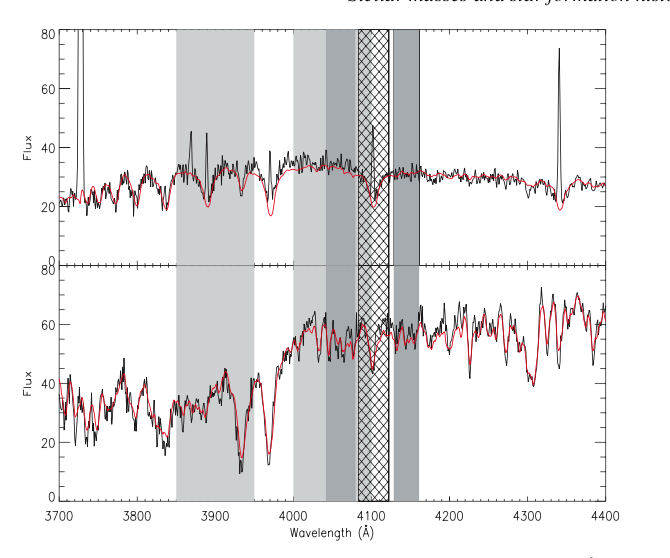
\includegraphics[width=\textwidth]{figures/spectra_placeholder.png}
\caption[PLACEHOLDER FIG; TBD: A figure showing D4000 and Hdelta breaks in spectra for early/late-type galaxies as well as the bimodality in D4000
]{ PLACEHOLDER FIG; TBD: A figure showing D4000 and Hdelta breaks in spectra for early/late-type galaxies as well as the bimodality in D4000
\label{fig:early_late_type}}
\end{figure}


\begin{figure}
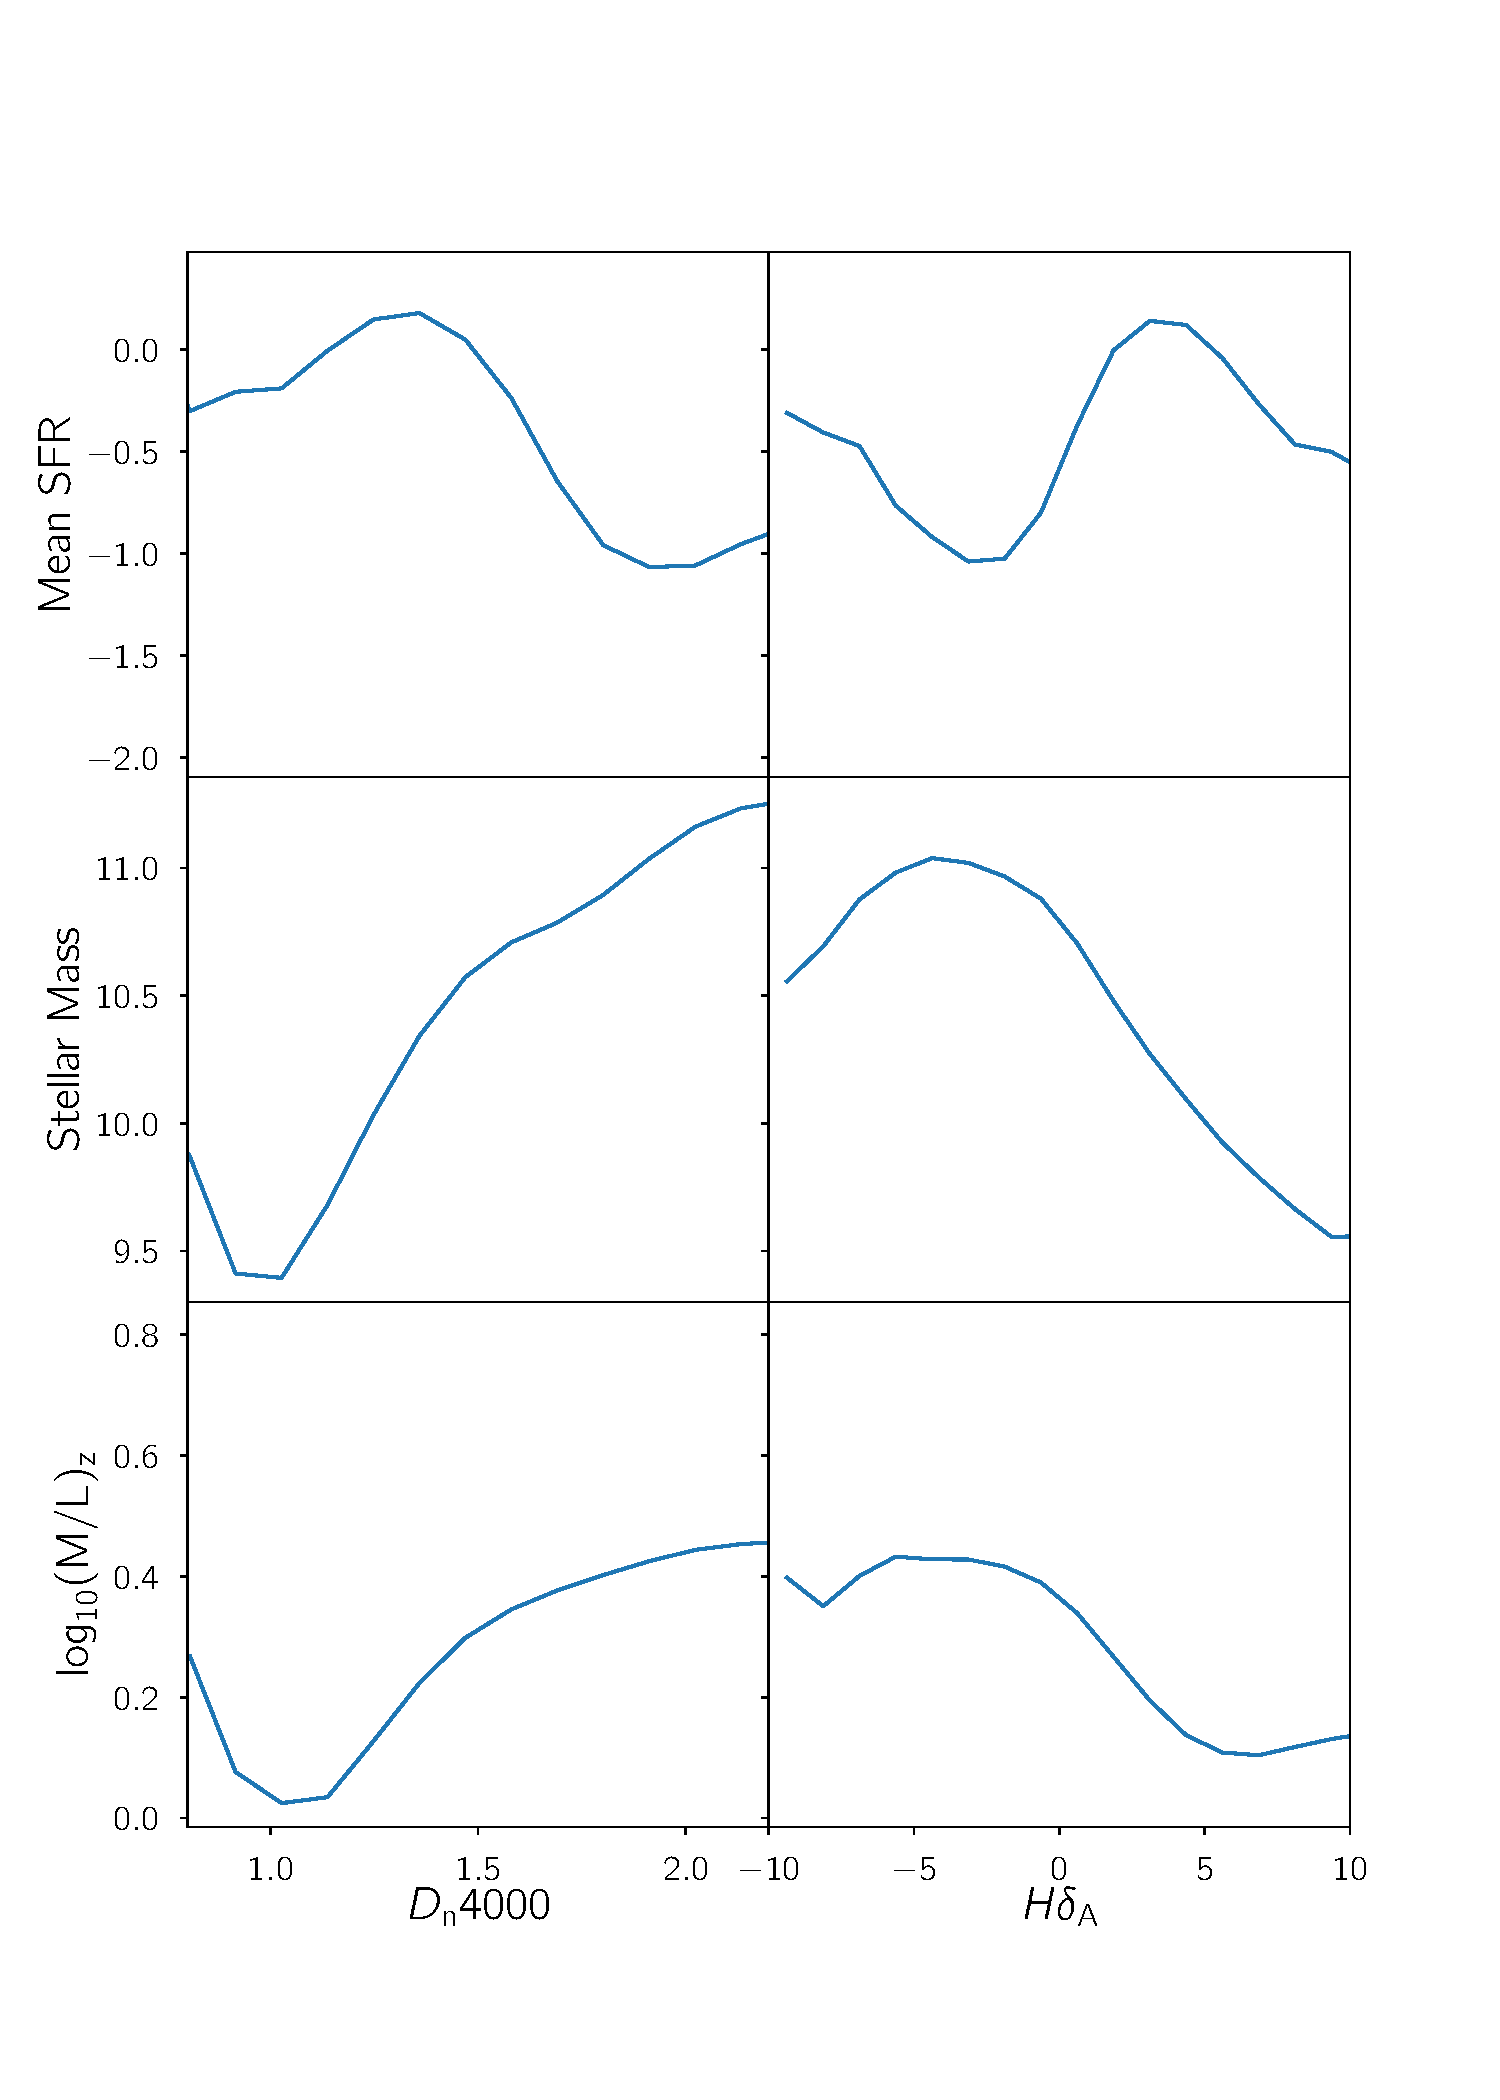
\includegraphics[width=\textwidth]{figures/mass_age_sfr_dist.pdf}
\caption[The \citet{kauffmann_stellar_2003} grid to infer M/L ratios from the $h\delta_{A}-D_{n}4000$ plane]
{The \citet{kauffmann_stellar_2003} grid to infer M/L ratios from the $h\delta_{A}-D_{n}4000$ plane
\label{fig:kauff_grid}}
\end{figure}


\subsection{The Balmer H$\delta$ Absorption Line}
\label{hdelta}

As we have seen in Section \ref{sed}, the spectral features of galaxies contain a wealth of information about their star formation properties. In particular the Balmer lines in the optical are very useful in understanding the ionized hydrogen content in the stellar populations in the galaxies and can thus provide valuable insight into star formation properties. The Balmer emission lines are the result of re-emission of light from hot, young stars by the ISM or HII regions in galaxies as we have seen in Section \ref{sfrs}. The absorption lines such as the H$\beta$, H$\gamma$ and H$\delta$ absorption lines, however, are characteristic of stellar spectra (predominantly occurring in A-type stars) and are thus tracers of the age and metallicity of stellar populations in galaxies. In particular, a strong H$\delta$ absorption feature is indicative of a starburst having happened 0.5-1.5 Gyrs ago \citep{1983ApJ...270....7D}, assuming that the stellar populations involved are mostly A-type stars.\\

The evolution of the Balmer absorption line profiles in stellar spectra with age points to a tendency for the width of the lines to increase with the age of the stars until about 0.5 Gyr for stellar populations with solar metallicity. Up until ages of about 1 Gyr, the Balmer lines of individual stars are not dependent on metallicity. However the interpretation of stellar age from the integrated light from stellar populations can still be affected by metallicity considerations as lower metallicity stars evolve more slowly in the HR diagram with the strength of the absorption feature peaking at ages older than 1 Gyr. Thus a lower metallicity stellar population at an older age would exhibit a similar H$\delta$ absorption feature as an intermediate-age stellar population with solar (or higher) metallicity.\\

The distinguishing factor, however, in the way the age-metallicity degeneracy affects the Balmer lines as opposed to the metallic absorption features is that the latter is tied more to the presence of the red giant branch stars and the former is more a consequence of the dependence of the main sequence turnoff temperature being a function of metallicity. Thus with the appropriate SPS models, both the mean age and metallicity can be simultaneously obtained. Particularly useful in this endeavor are the Lick indices, obtained by using stellar spectra from the Lick Observatory \citep{1997ApJS..111..377W, worthey_comprehensive_1994}. The Lick indices are a system of 25 line indices, that can successfully disentangle the effects of age and metallicity for a given [$\alpha$/Fe] abundance ratio.\\ 

Measuring an absorption feature involves measuring the flux in a central bandpass relative to two pseudo-continuum bandpasses on either side. A line is drawn between the midpoints of the two flanking pseudo-continuum bandpasses to define the continuum from which an equivalent width is measured by integration. The bandpass definitions we use here, as defined by \citet{worthey_comprehensive_1994} are: an index Bandpass from 4083.50 - 4122.25 \AA with the blue and red bandpasses on either side being 4041.60 - 4079.75 \AA and 4128.50 - 4161 \AA respectively.

\subsection{Constraining SFH's using H$\delta_{\rm A}$ and $D_{\rm n}4000$}
\label{kauffmann method}

The methods used by \citep{kauffmann} involve fitting observed spectra with SPS models based on spectral libraries to develop maximum likelihood estimated of stellar mass, star formation rates and stellar ages for the population of galaxies. Key to this is modelling the time evolution of a galaxy in the ${\rm H}\delta_{\rm A}$ - ${\rm D}_{\rm n} 4000$ phase space. As it turns out, together, these two indices provide a significant observational constraint on the age of a a galaxy. Even though the time evolution of either indicator in isolation does indeed depend on metallicity, the locus of galaxies in the plane is not as sensitive to metallicity and is informative of whether or not a star burst episode

\subsection{The MPA-JHU Aperture Correction/Aperture Bias}
\label{apercorr}


\begin{figure}
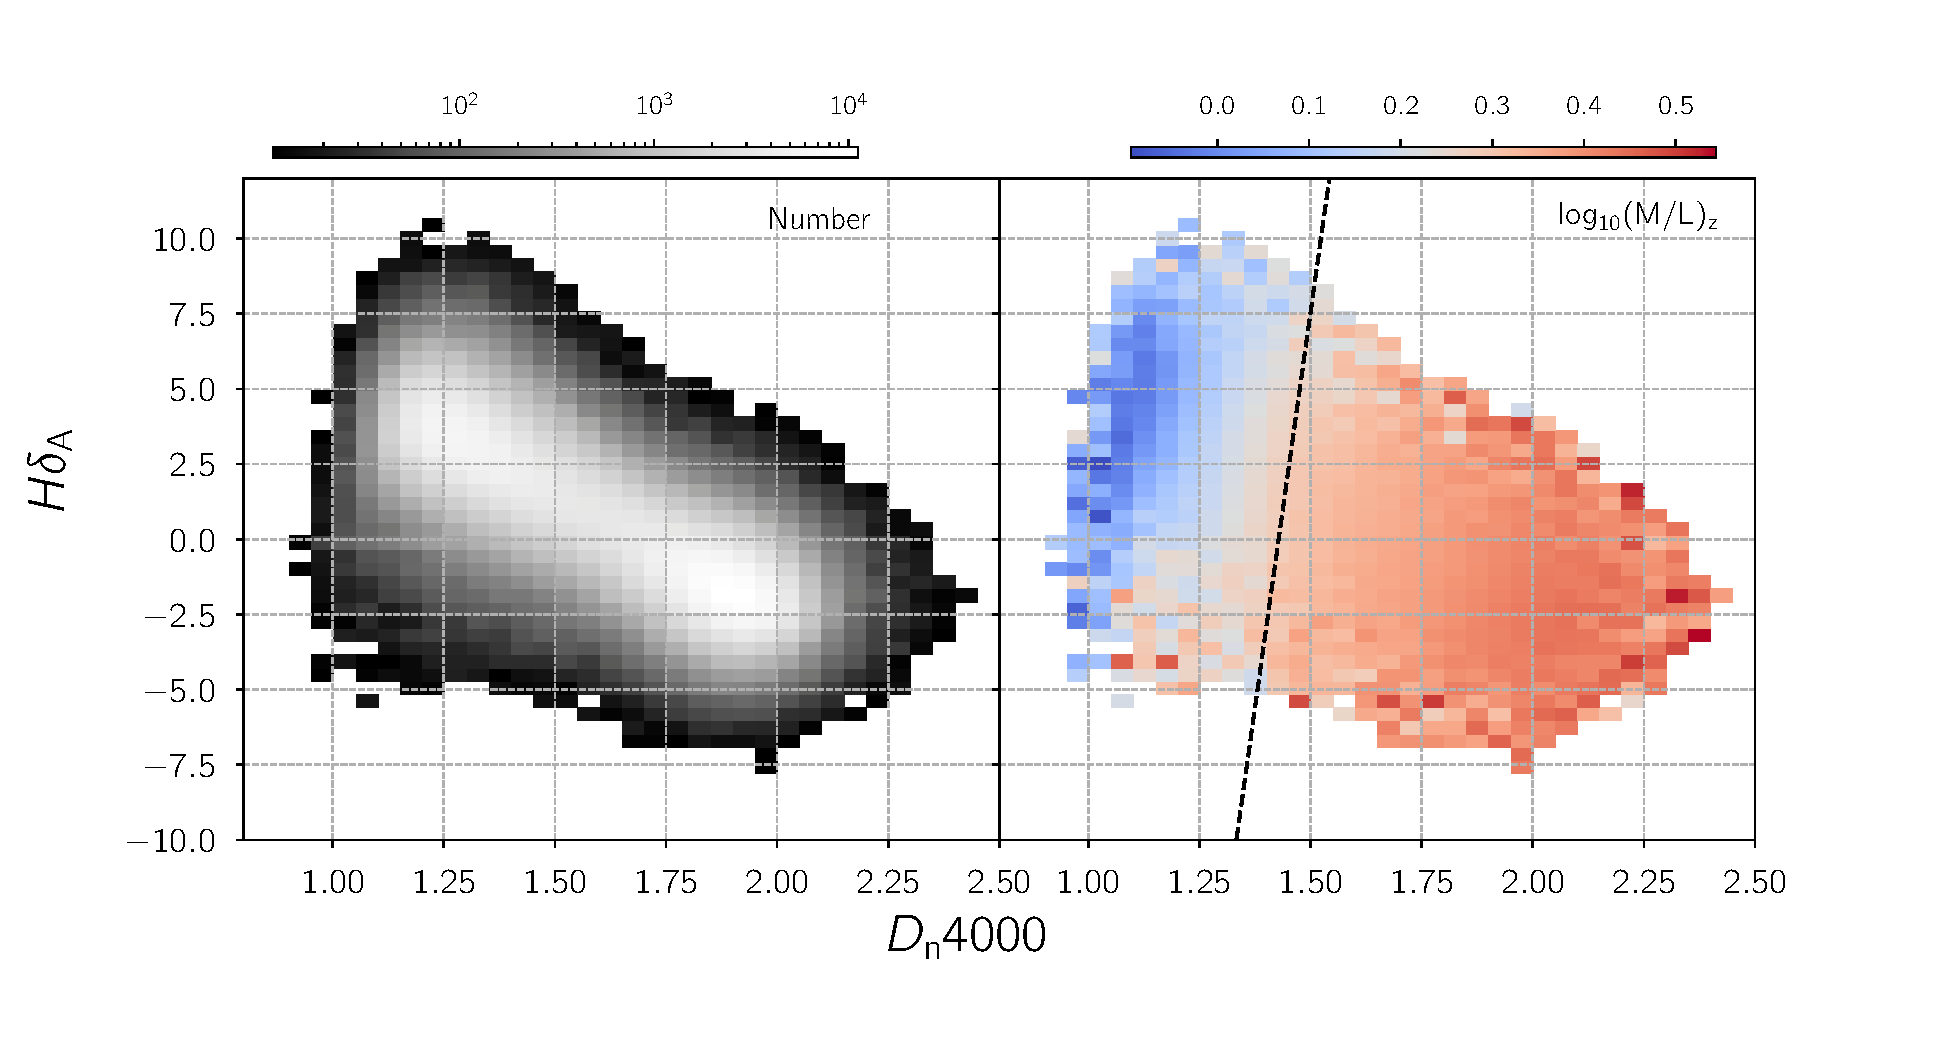
\includegraphics[width=\textwidth]{figures/hd_d4000_mlratio_coarser_binning.pdf}
\caption[The \citet{kauffmann_stellar_2003} grid to infer M/L ratios from the $h\delta_{A}-D_{n}4000$ plane]
{The \citet{kauffmann_stellar_2003} grid to infer M/L ratios from the $h\delta_{A}-D_{n}4000$ plane
\label{fig:kauff_grid}}
\end{figure}



\section{Data}

\subsection{MaNGA Target Selection and DRP}
\label{mangadrp}
Primary and Secondary Samples. NSA redshifts/Luminosity cut.

\subsection{Our Sample}
The most recent MaNGA product launch, MPL-$8$, which was announced in November $2018$, containing products based on galaxy and stellar library observations from March $2014$ - July $2018$ serves as the source of our sample. It contains $950$ plates - $6779$ data cubes and $20649$ stellar library stars. Out of these, $6468$ are galaxies with measured NSA redshifts. These are representative of all the IFU sizes (list them: 19,37... 127) and span a redshift range upto $z = 0.15$.\\
For each galaxy observation, depending on the IFU bundle size (say $N_{X}$, $N_{Y}$ each describing a position $0.5$" from the previous spaxel), we have ($N_{X}$, $N_{Y}$) spectra which span $4563$ wavelength points. 

\section{Methods}
\label{sec:chap2methods}

\subsection{Variable Aperture Measurements}
For any given datacube, we can determine which spaxels fall within an aperture radius of $R$ arc-seconds as follows. As each spaxel spans a width of 0.5'' in along the ``X" and ``Y" direction, at any point $(x,y)$ in the IFU image, the distance in arc-seconds of the centre of a spaxel from the central spaxel $(x_{c},y_{c})$ in the IFU would be:
$$ d = (r(x,y) - r(x_{c},y_{c})) = \sqrt{(0.5*x)^2 + (0.5*y)^2} $$
Thus, for every spaxel in the IFU, where $d<=R$, that part of the galaxy would fall within the aperture and hence, we would include that spaxel in the measurement of whichever spectral index. Using this, for instance, we can simulate the SDSS fiber measurement, i.e.,  what the $1.5$" aperture radius used in SDSS would see versus the total galaxy or what we call a ``full aperture" measurement.

%\begin{figure}
%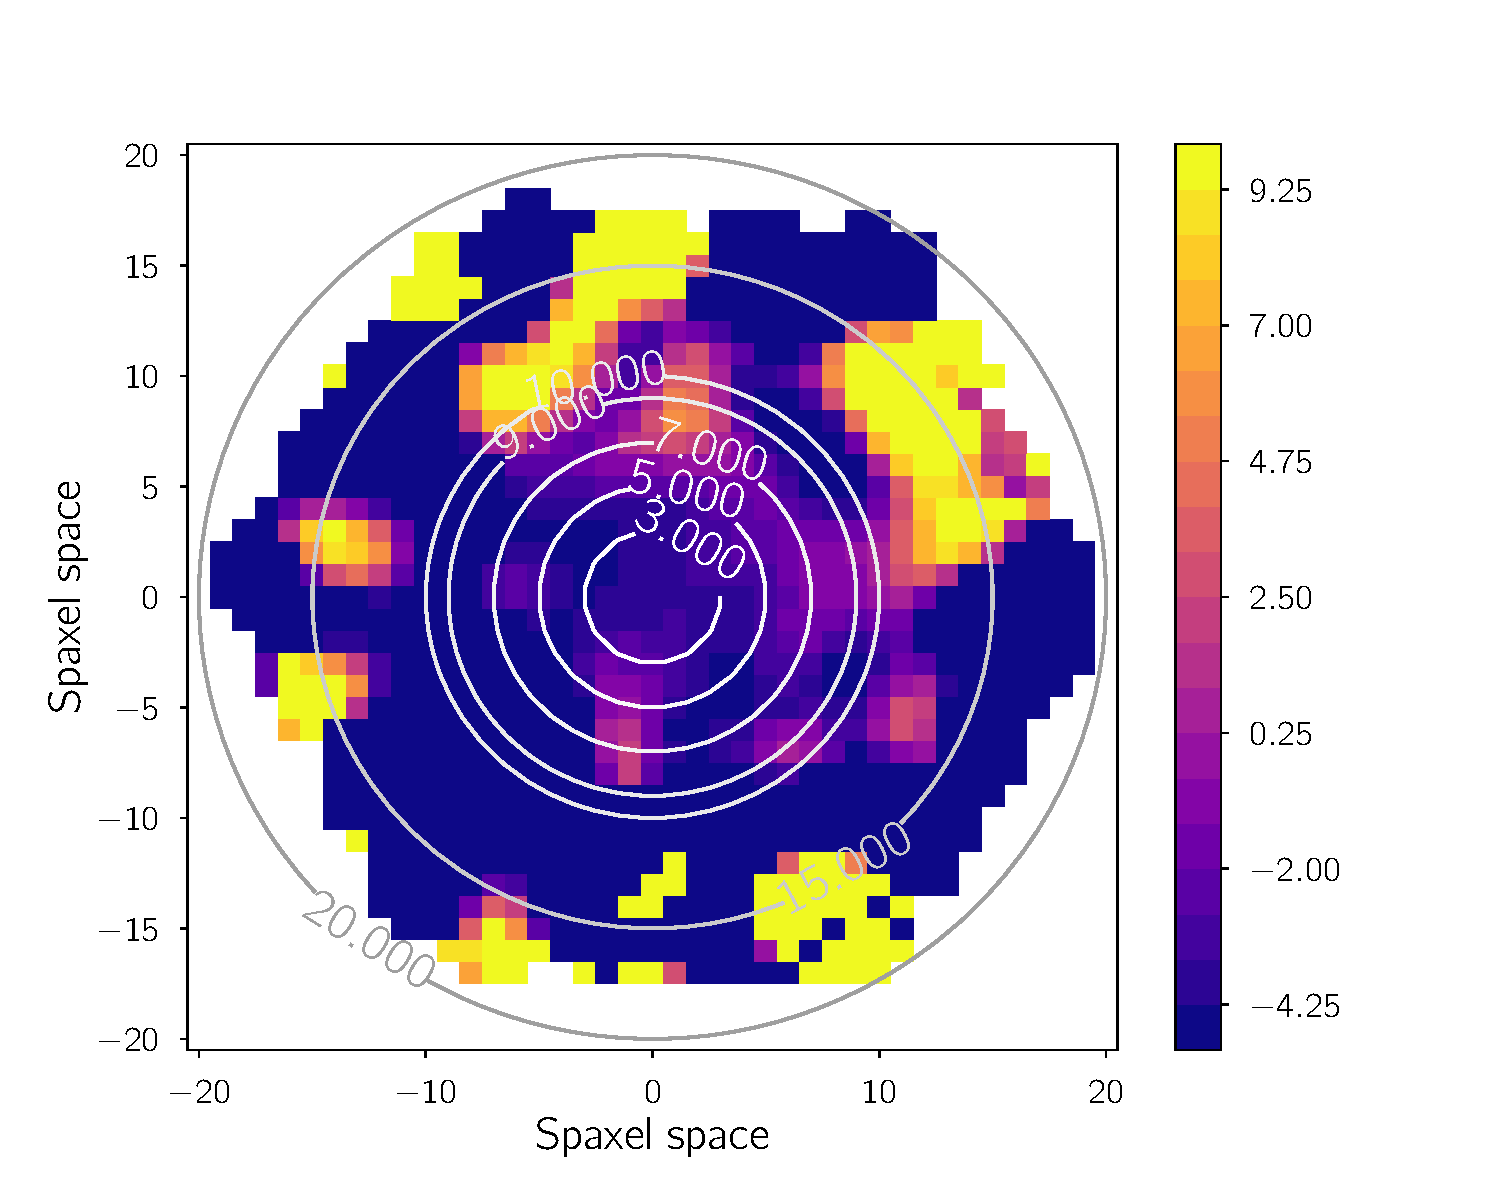
\includegraphics[width=\textwidth]{figures/gal_aperture.pdf}
%\caption[Placeholder figure: TBD. Sample MaNGA galaxy view in the spaxel space with the $H{\delta_{\rm A}}$ distribution plotted as a function of position and the contours marking the aperture diameters at different angular distances in arcseconds]
%{Placeholder figure: TBD. Sample MaNGA galaxy view in the spaxel space with the $H_{\delta_{\rm A}}$ distributions plotted as a function of position and the contours marking the aperture diameters at different angular distances in arcseconds
%\label{fig:sample_manga}}
%\end{figure}

One can alternately pose this question in terms of redshift. For all galaxies whose redshift $z_{\rm obs}$ is less than the redshift we are interested in, $z_{\rm cutoff}$, we can ask the question: if we shift the said galaxy to the said cutoff point, where would its location on the $H\delta_{\rm A}$ - $D_{\rm n}4000$ plane be? How offset is this from the ``full aperture" measurements?\\

Transverse angular distance varies with redshift as follows:
$$D_{\rm A}(z) = \frac{D_{\rm M}(z)}{1+z} $$,
where $D_{\rm M}(z)$ is the co-moving distance at redshift z.

So when a galaxy at $z_{\rm obs}$ is shifted to $z_{\rm cutoff}$ the new distance $d_{\rm new}$ of spaxel $(x,y)$ from the central spaxel $(x_{c},y_{c})$ relates to the old distance thus:
$$ d_{\rm new} = \frac{(1+z_{\rm cutoff})\times D_{\rm M}(z_{\rm obs}) \times d}{(1+z_{\rm obs}) \times  D_{\rm M}(z_{\rm cutoff})} $$

Using the above, we can now figure out the spaxels that would fall within a 3'' diameter aperture (say) at not only the observed redshift but also any redshift where we would like to collectively observe the behavior of the offset with a full aperture measurement in the $H\delta_{\rm A}$ - $D_{\rm n}4000$ plane.

\begin{figure}
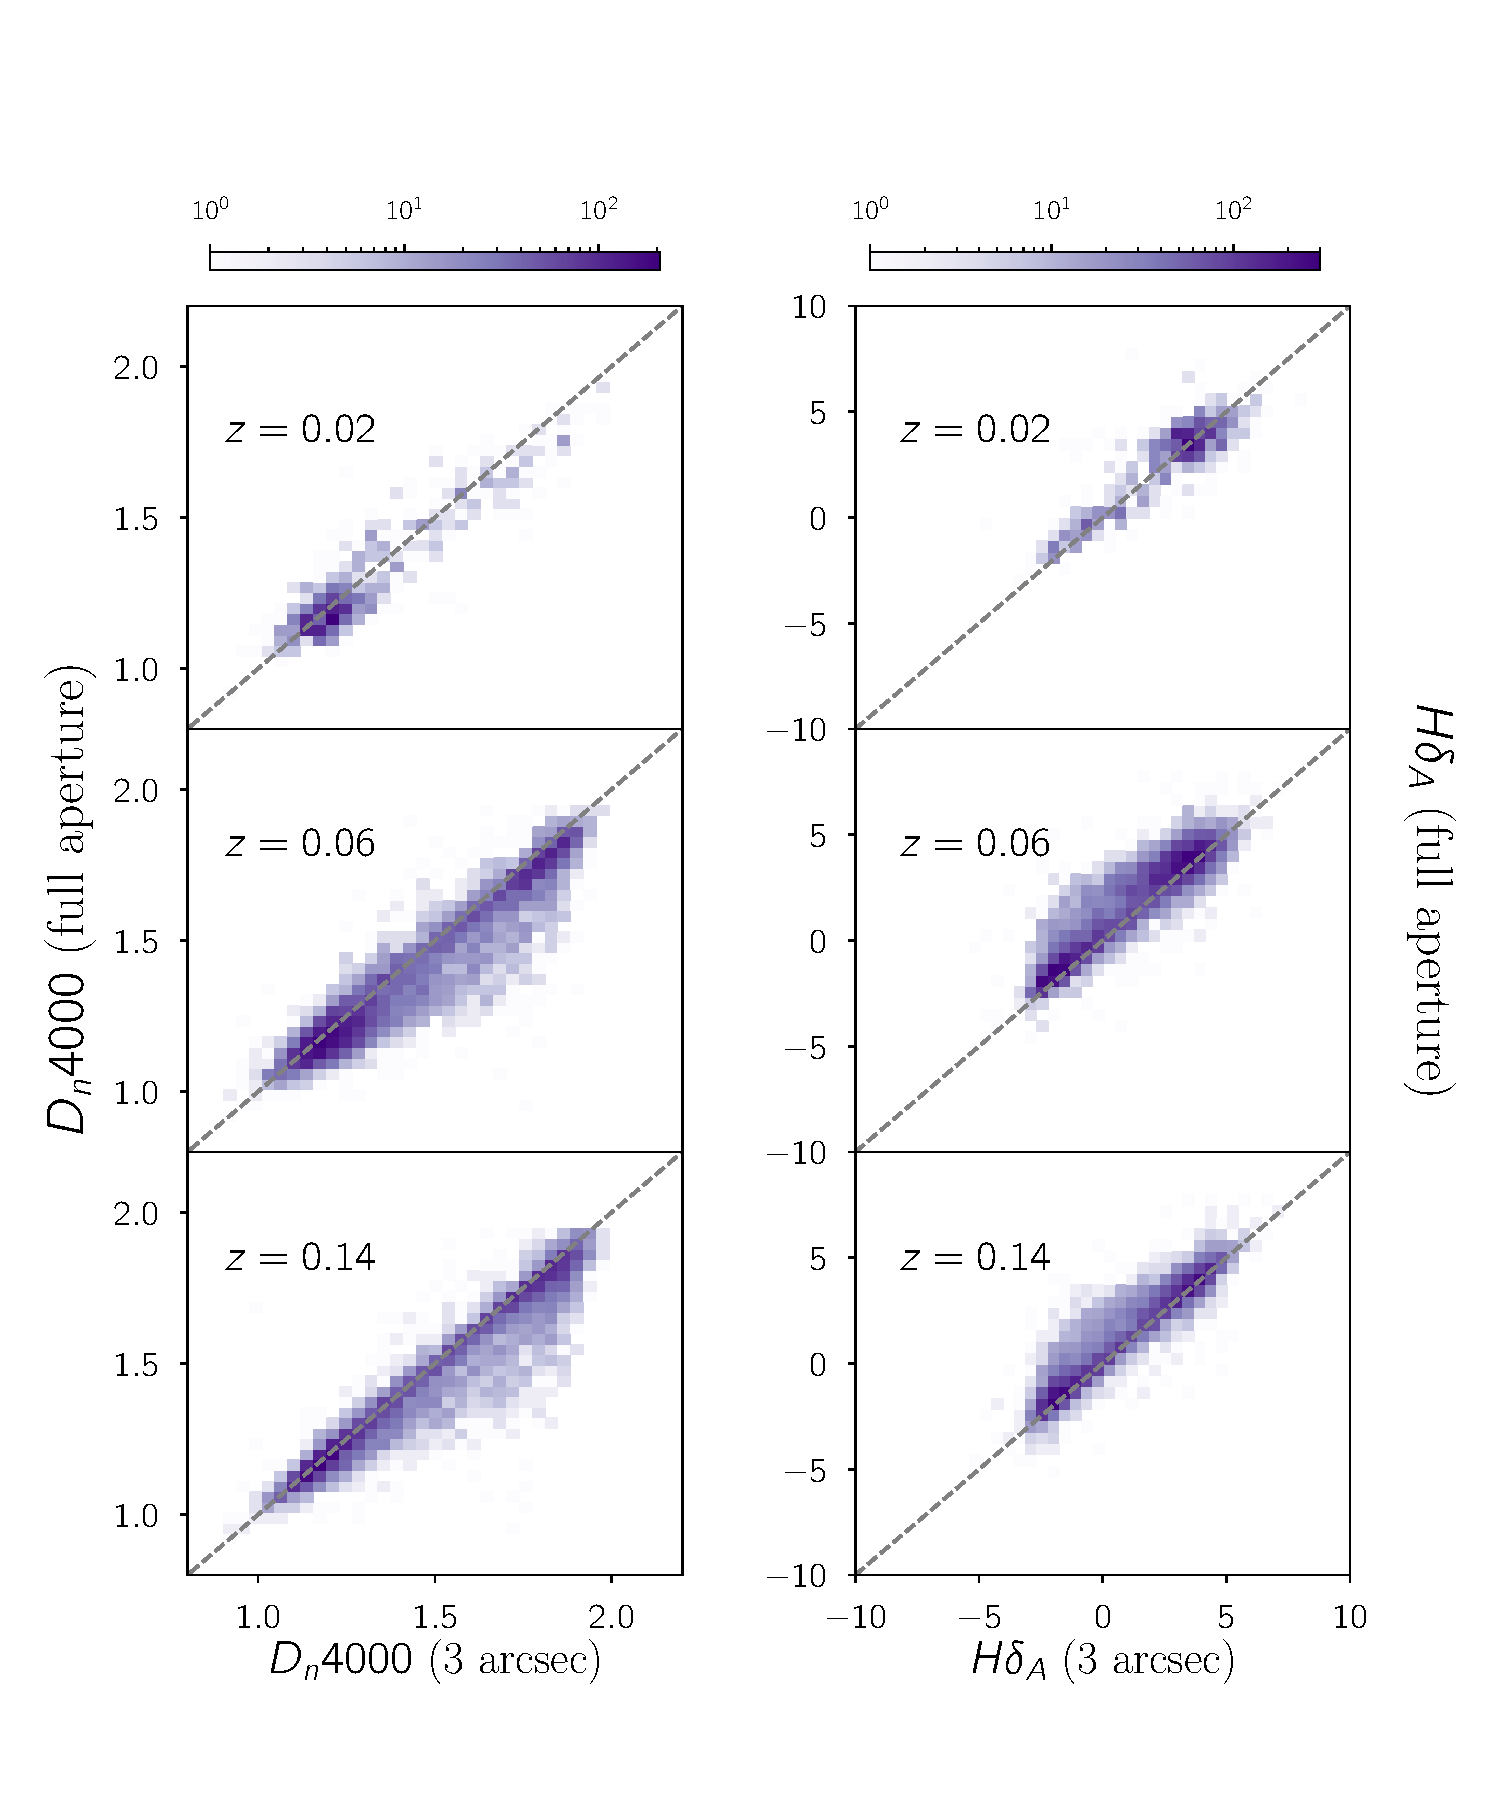
\includegraphics[width=\textwidth]{figures/full_aperture_comparisons.pdf}
\caption[The $D_{n}4000$, $h\delta_{A}$ indices measured at $z = 0.02,0.06,0.14$ with a $3''$ aperture compared to the full aperture measurement]
{ The $D_{n}4000$, $h\delta_{A}$ indices measured at $z = 0.02,0.06,0.14$ with a $3''$ aperture compared to the full aperture measurement
\label{fig:redshift_comparison}}
\end{figure}


\subsection{$H\delta_{\rm A}$, $D_{\rm n}4000$ Measurements within Apertures}
To get the $H\delta_{\rm A}$ and $D_{\rm n}4000$ index measurements for any aperture, we first redshift-correct the spectra obtained from all the spaxels within the aperture to rest-frame. As both the equivalent width of the Balmer $H\delta$ line as well as the $D_{n}4000$ break rely on the continuum as well as a ratio of fluxes in the case of the latter, we add up the spectra of the spaxels that fall within any aperture before estimating either. We then follow the procedure described in Section $2.2$ to calculate the indices. (In a footnote: the code for this is publicly available at --provide github link--.)

\section{Results}
\subsection{Comparison to Full Aperture Measurements}
To investigate how the full aperture measurements compare to the 3'' measurements, we choose 3 different redshift bins $z = 0.02,0.06$ and $0.14$ and observe how offset the $H\delta_{\rm A}$ and $D_{\rm n}4000$ measures are. For each redshift, I pick the galaxies whose redshift are below that redshift and ``shift" them to the cutoff redshift as described in Section \ref{sec:chap2methods} and compare the full aperture measurements to the 3'' measurements made at that redshift. The results of this are shown in Fig. \ref{fig:redshift_comparison}, where the full aperture measurements are plotted against the 3'' measurements at the respective redshifts with the colorbars indicating the number of galaxies in each bin. We note that the total number of galaxies in each redshift bin is 561 for $z = 0.02$, 5016 for $z = 0.06$ and 6402 for $z = 0.14$.\\

\begin{figure}
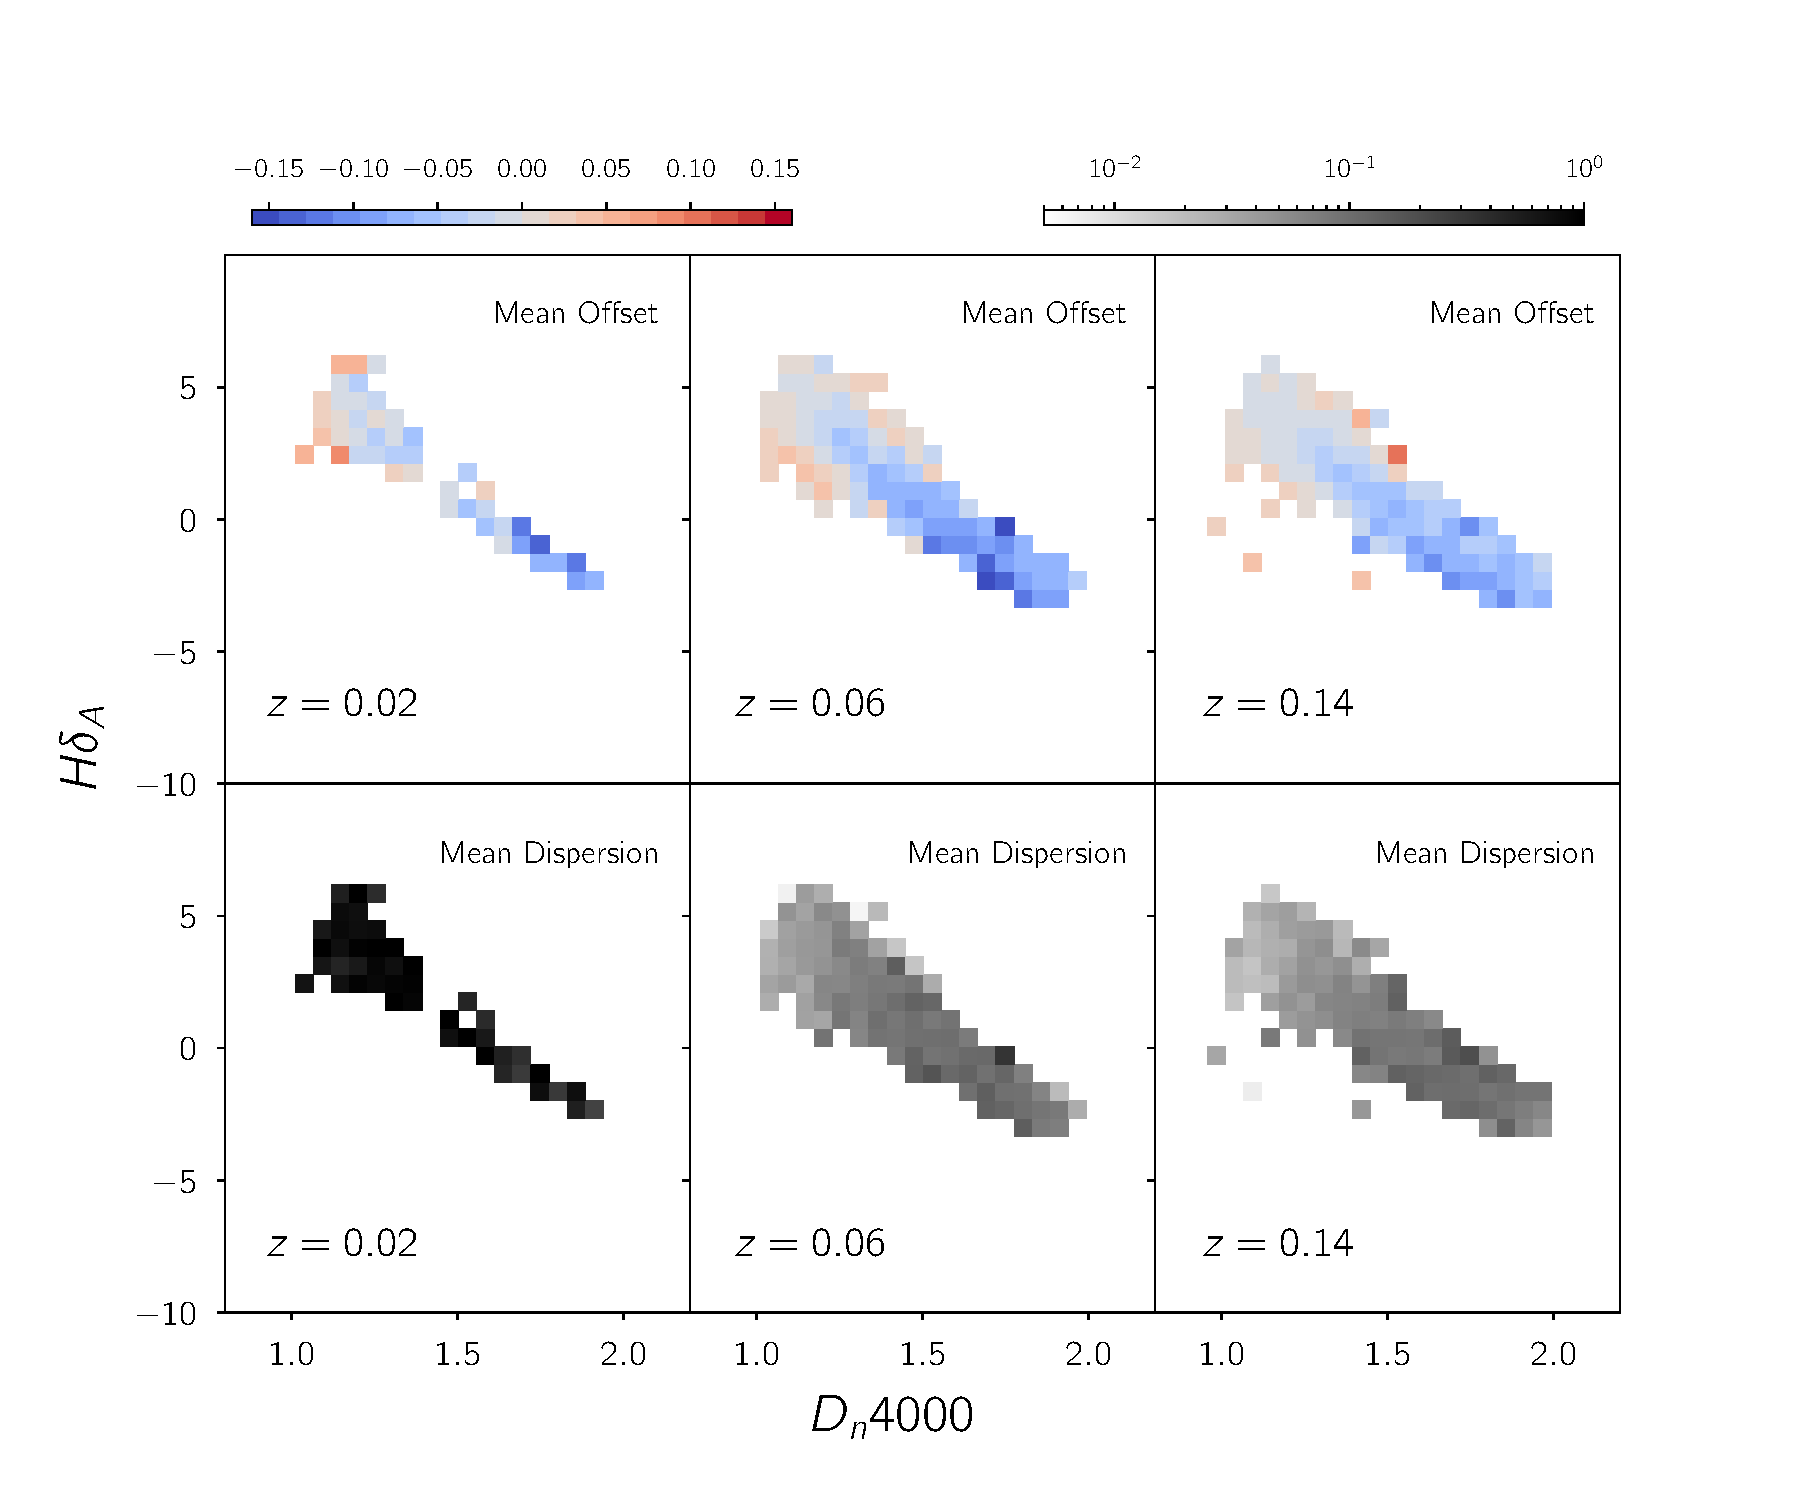
\includegraphics[width=\textwidth]{figures/dn4000_full_aperture_comparisons.pdf}
\caption[The mean offset and dispersion in the $D_{n}4000$ index measured at $z = 0.02,0.06$ and $0.14$ with a $3''$ aperture from the full aperture measurement]{ The mean offset and dispersion in the $D_{n}4000$ index measured at $z = 0.02,0.06$ and $0.14$ with a $3''$ aperture from the full aperture measurement
\label{fig:offset_d4000}}
\end{figure}

From Fig. \ref{fig:redshift_comparison}, we can infer the following. For most of the galaxies the offset is pretty minimal as it as they fall pretty close to the $x=y$ line. We find that the scatter is the most at $z = 0.06$ and tends towards higher $D_{\rm n}4000$ and lower $H\delta_{\rm A}$ values relative to the full aperture measurements. This can be interpreted as the effect of the apertures beginning to cover the galaxy disks which have lower star formation activity than the bulge for galaxies with strong bulges. The scatter lessens as we approach $z = 0.14$, close to the survey limit, where for most of the galaxies, all of the light gets accounted for by the 3''aperture at this point.\\

\begin{figure}
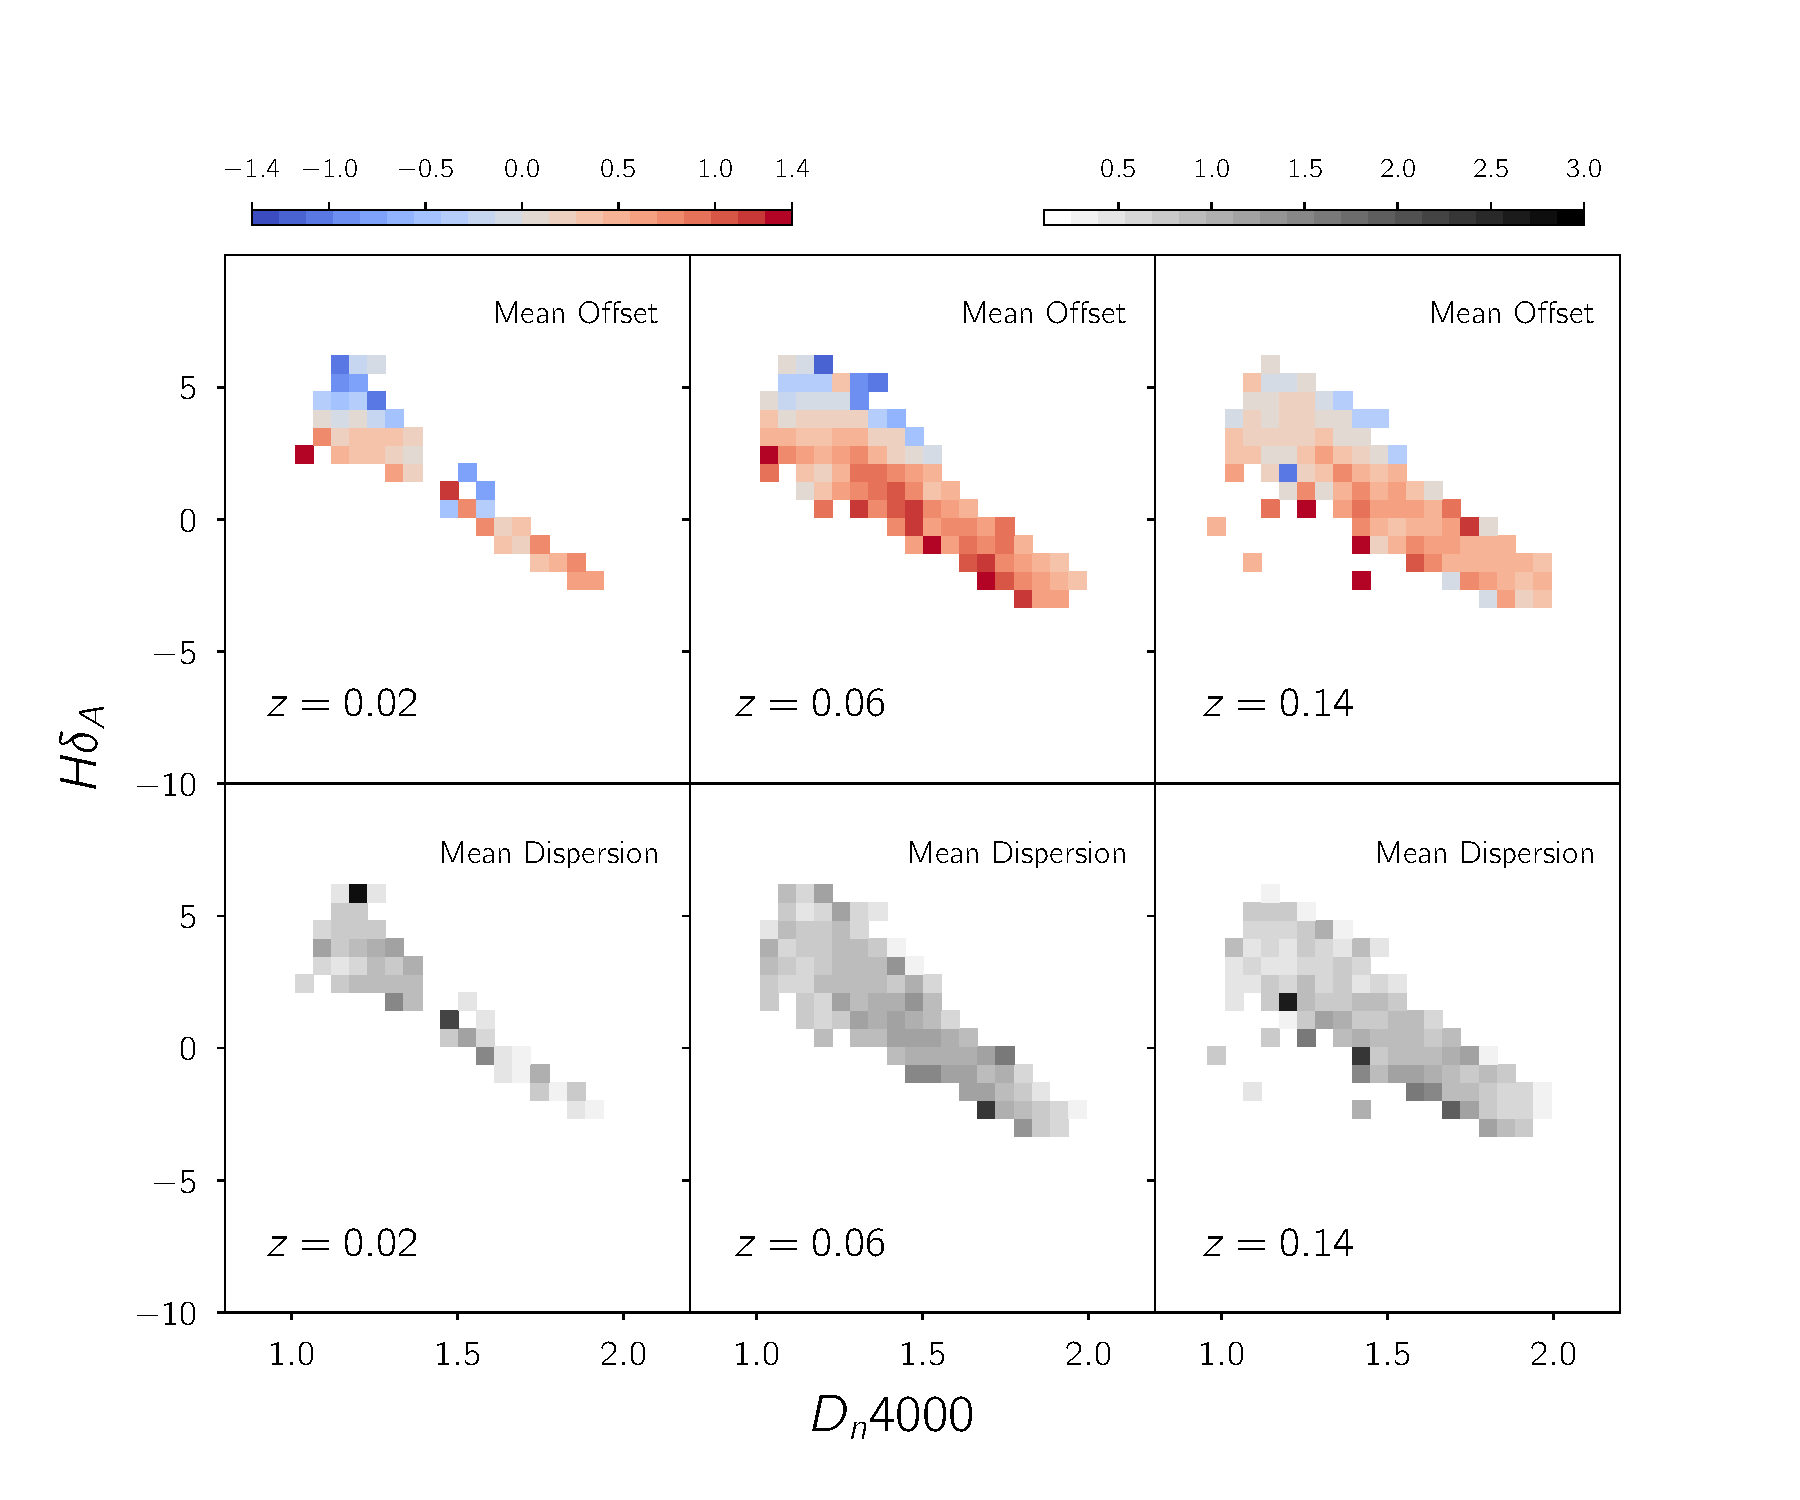
\includegraphics[width=\textwidth]{figures/hdelta_full_aperture_comparisons.pdf}
\caption[The mean offset and dispersion in the $h\delta_{A}$ index measured at $z = 0.02,0.06$ and $0.14$ with a $3''$ aperture from the full aperture measurement ]{ The mean offset and dispersion in the $h\delta_{A}$ index measured at $z = 0.02,0.06$ and $0.14$ with a $3''$ aperture from the full aperture measurement 
\label{fig:offset_hdelta}}
\end{figure}

MRB Says: At all redshifts, we can see that there is a systematic tendency for galaxies to appear older through the fiber aperture than through the full aperture, and therefore to appear to have a higher M/L than they actually do. This would particularly affect the intermediate age galaxies (i.e. those with $D_{\rm n}4000$ in the green valley).\\


\subsection{Offsets in the $H\delta_{\rm A}$-$D_{\rm n}4000$ plane}

\begin{figure}
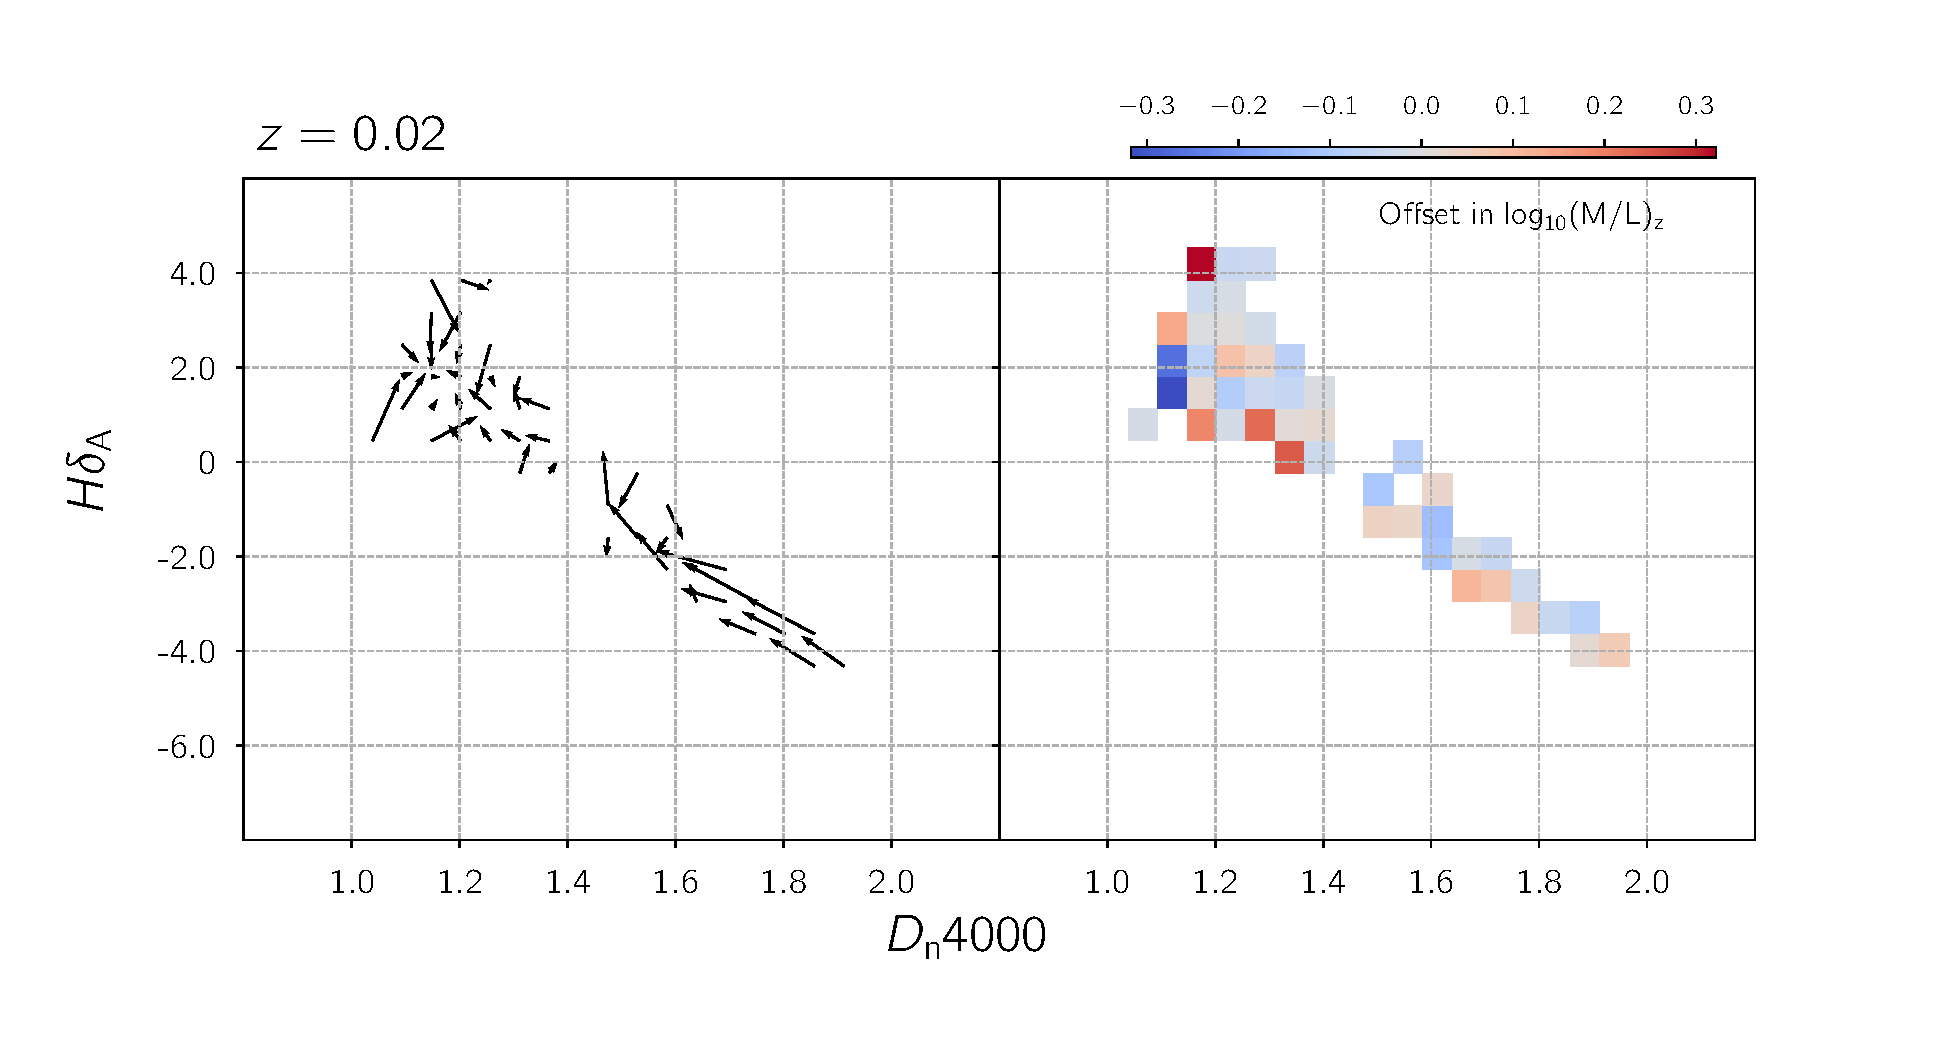
\includegraphics[width=\textwidth]{figures/mlz_offset_a.pdf}
\caption[ The combined mean offset in $D_{\rm n}4000$-$h\delta_{\rm A}$ at $z=0.02$ from the full aperture measurements represented as a vector whose projections on the axes are the actual offsets in either direction ]{ The combined mean offset in $D_{\rm n}4000$-$h\delta_{\rm A}$ at $z=0.02$ from the full aperture measurements represented as a vector whose projections on the axes are the actual offsets in either direction
\label{fig:offset_quiver1}}
\end{figure}


\begin{figure}
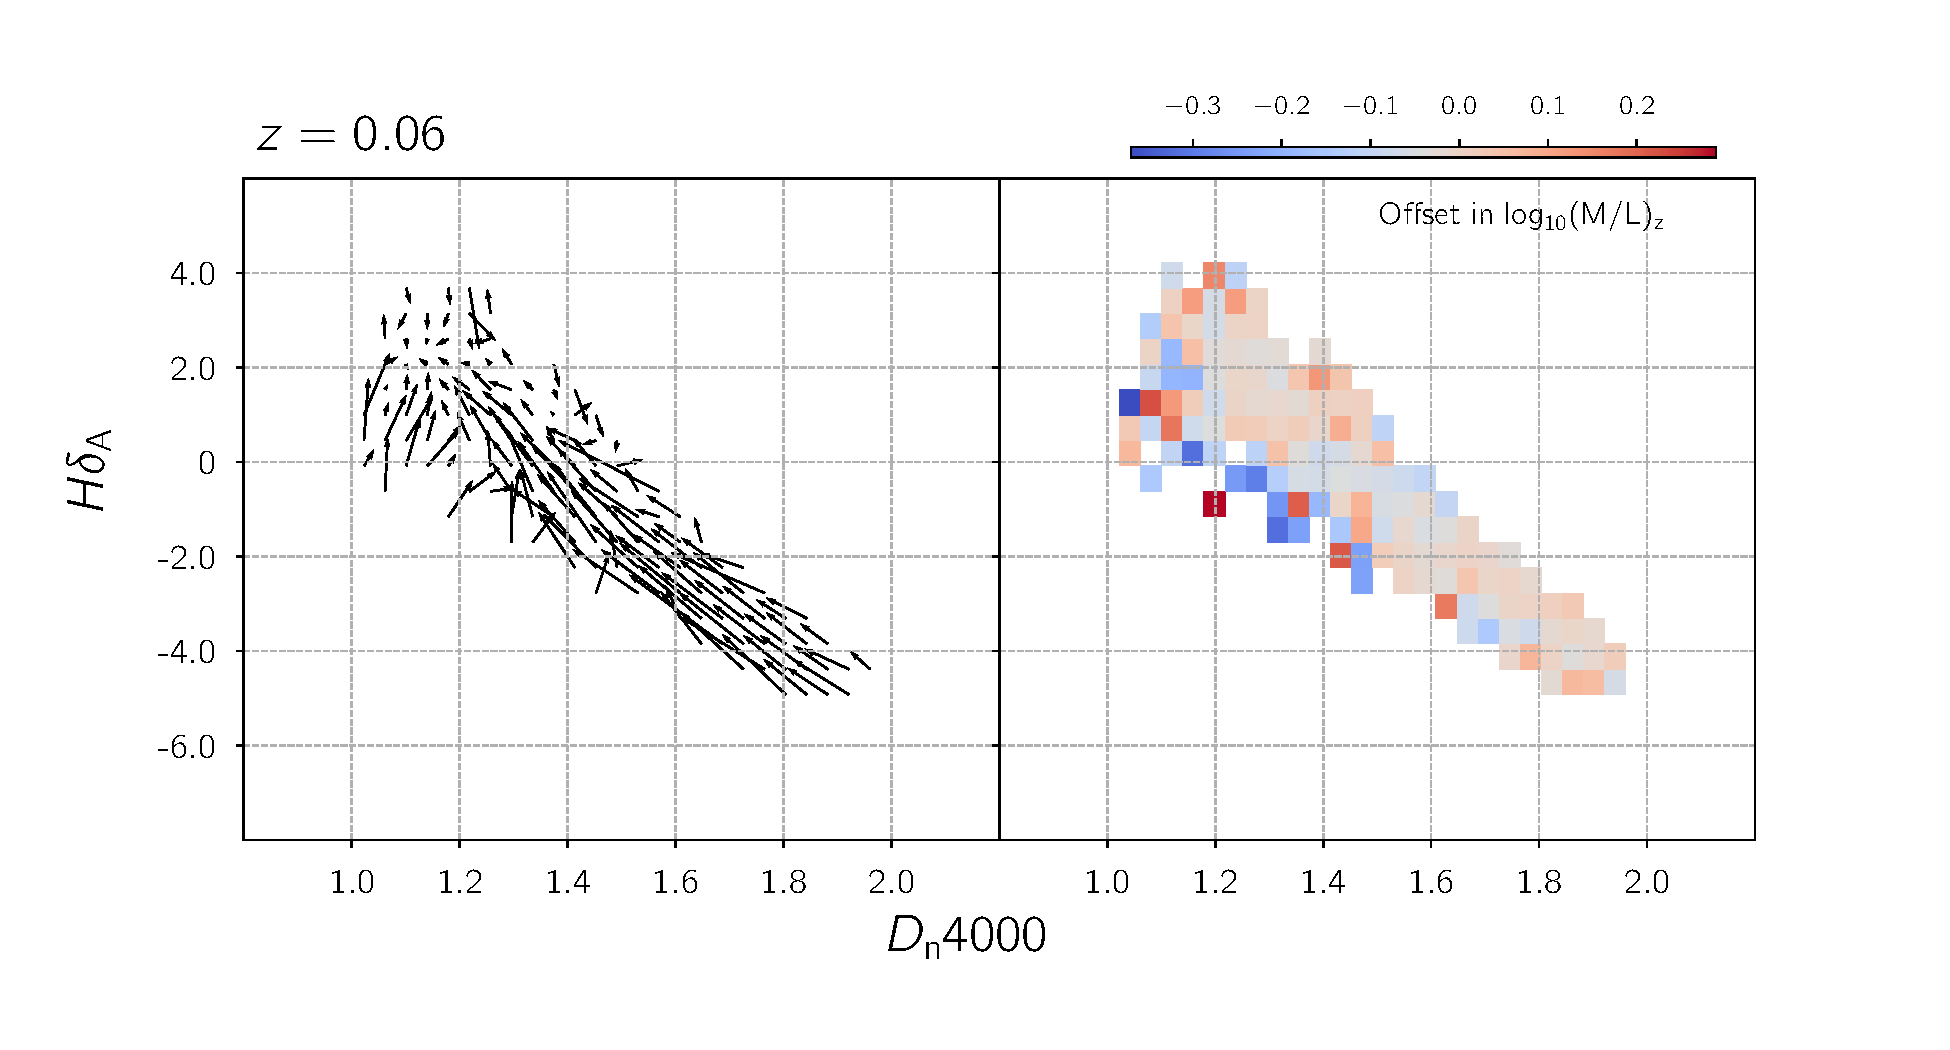
\includegraphics[width=\textwidth]{figures/mlz_offset_b.pdf}
\caption[ The combined mean offset in $D_{\rm n}4000$-$h\delta_{\rm A}$ at $z=0.06$ from the full aperture measurements represented as a vector whose projections on the axes are the actual offsets in either direction ]{ The combined mean offset in $D_{\rm n}4000$-$h\delta_{\rm A}$ at $z=0.06$ from the full aperture measurements represented as a vector whose projections on the axes are the actual offsets in either direction
\label{fig:offset_quiver2}}
\end{figure}

\begin{figure}
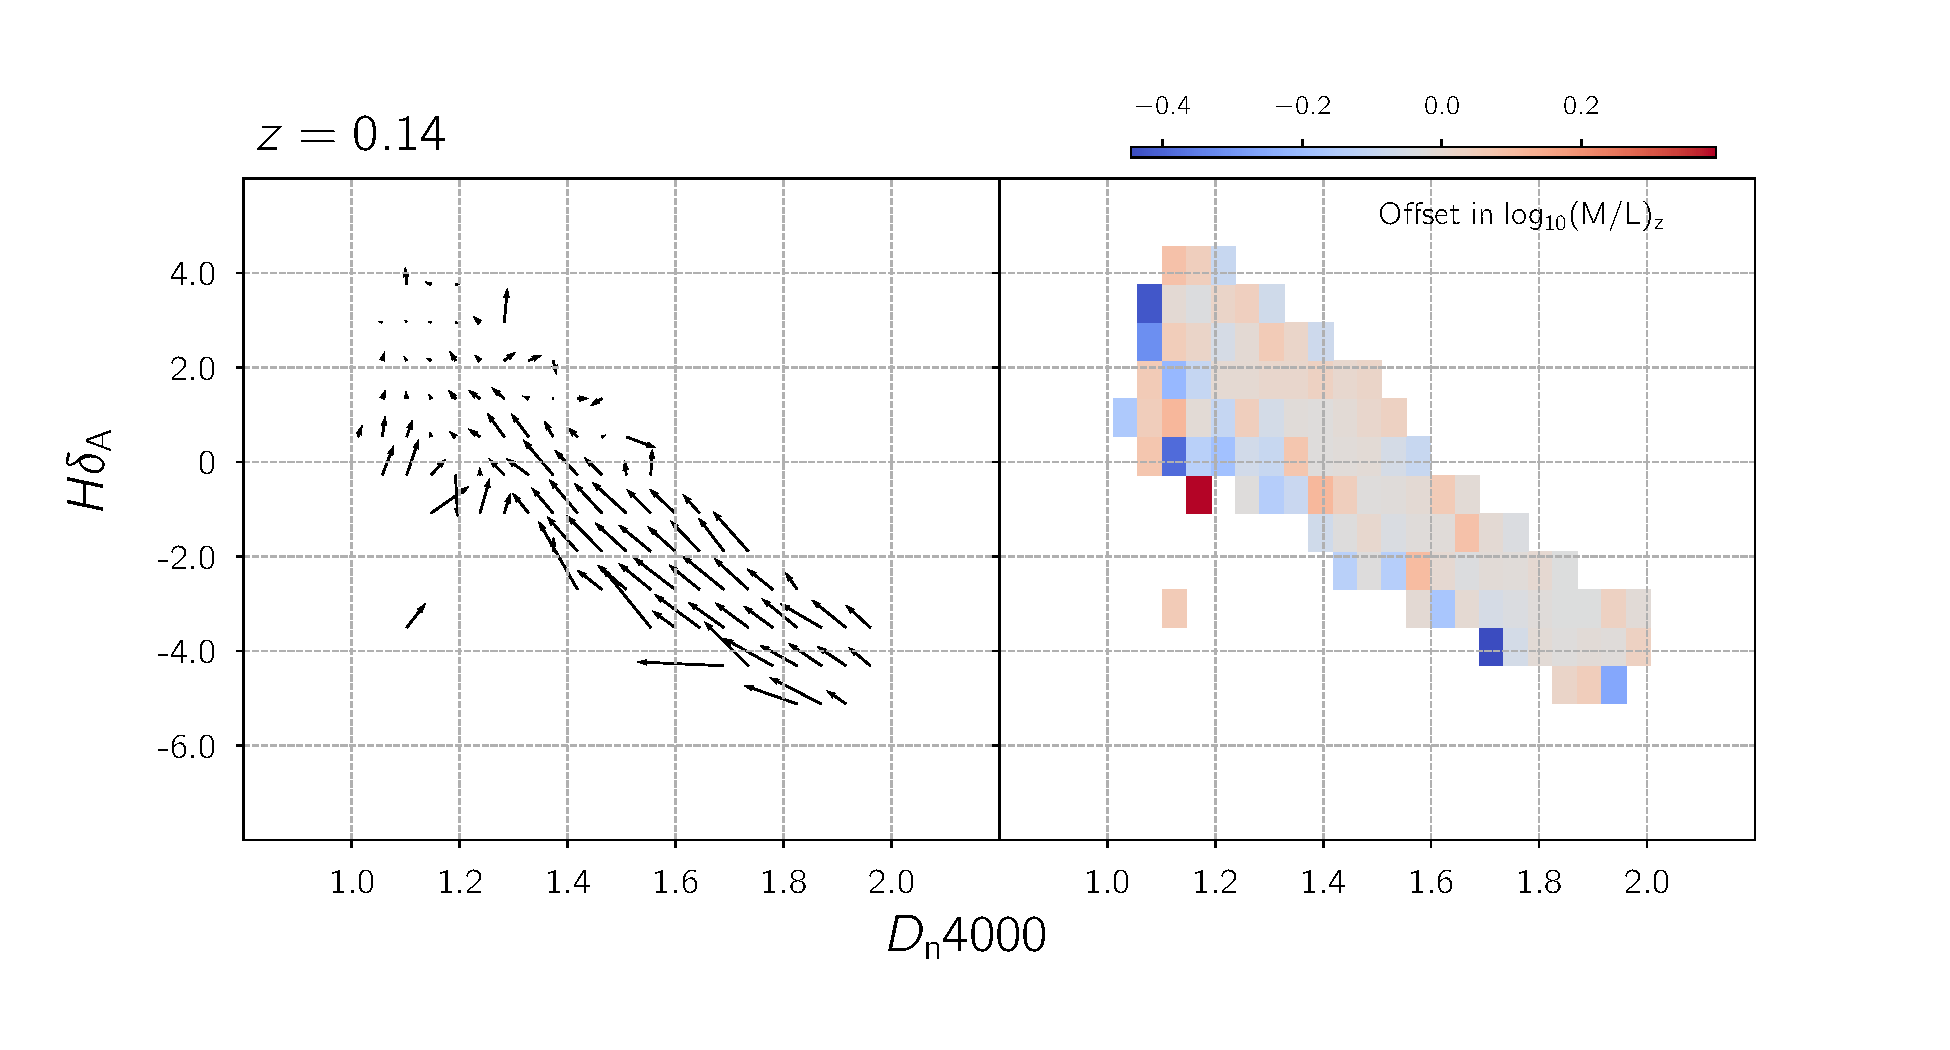
\includegraphics[width=\textwidth]{figures/mlz_offset_c.pdf}
\caption[ The combined mean offset in $D_{\rm n}4000$-$h\delta_{\rm A}$ at $z=0.14$ from the full aperture measurements represented as a vector whose projections on the axes are the actual offsets in either direction ]{ \emph{Left:} The combined mean offset in $D_{\rm n}4000$-$h\delta_{\rm A}$ at $z=0.14$ from the full aperture measurements represented as a vector whose projections on the axes are the actual offsets in either direction. \emph{Right:} The offsets transformed to the z-band mass-to-light ratios using 
\label{fig:offset_quiver3}}
\end{figure}

\section{Discussion}

MRB Says: * This mean tendency is *relatively* small. You should calculate from your grids the median offset for cells with D4000 > 1.3 or something like that, and quote that number. You should then look carefully at the Kauffmann figure to translate this to a change in $M/L_z$ --- my guess is that it is around 0.1 dex for z=0.06. Do this for z=0.06 and z=0.14.

 * The scatter about this mean is substantial relative to the mean. Again, calculate the median standard deviation over the cells with D4000 > 1.3 to quantify this. My guess is that it is  comparable to the mean itself. This means for individual galaxies the error can be a lot bigger. Again quote for both those redshifts.

 * The main conclusion is that stellar masses more accurate than 0.1 dex (or whatever you see in the mean offset) arenot possible, and that the scatter in the offset means the precision is degraded as well. This source of error is important
to keep in mind but is probably not fatal for samples at z=0.1
from MPA/JHU --- most results done rely on stellar masses
at that precision. Using this sample at lower redshift may be
much more iffy.







